\chapter{Background}
	
	\label{sec:background}
	
	\section{Super computers}
		
		\begin{figure}
			\center
			\buildrplot{figures/top500-num-processors.R}
			
			\caption{Historical processor (core) counts for the `Top500' super
			computer installations. The line shows the mean number of processsors and
			gray ribbon indicates the range. Data reported by the `Top500 List'
			\cite{meuer15j}.}
			\label{fig:top500-num-processors}
		\end{figure}
		
		Super computers have been growing in size at an exponential rate as we can
		see in figure~\ref{fig:top500-num-processors}.
		
		\subsection{Applications and architecture}
		\subsection{Network topology and construction}
		\subsection{Routing}
	
	\section{Neural modelling and simulation}
		\subsection{Neural modelling}
		\subsection{Spikes}
		\subsection{High-level modelling tools}
	
	\section{SpiNNaker}
		\subsection{Architecture}
		\subsection{Network topology}
		
			% TODO: Introduce topology
			
			% TODO: Reword the following lifted straight from wiring paper.
			
			\begin{figure}
				\center
				\buildfig{figures/hexagonalTorusTopology.tex}
				
				\caption{A $10 \times 10$ hexagonal torus topology with wrap-around
				links between $a$, $b$, $c$ and $a'$, $b'$, $c'$, respectively, omitted
				for clarity. The hexagonal torus's three non-orthogonal axes are shown
				in grey.}
				\label{fig:hexagonalTorusTopology}
			\end{figure}
			
			\begin{figure}
				\center
				\begin{subfigure}{0.39\linewidth}
					\center
					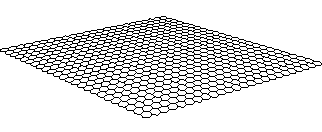
\includegraphics[width=\linewidth]{figures/torus-3d-flat.pdf}
					\caption{}
					\label{fig:torus-3d-flat}
				\end{subfigure}
				~~
				\begin{subfigure}{0.26\linewidth}
					\center
					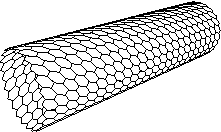
\includegraphics[width=\linewidth]{figures/torus-3d-tube.pdf}
					\caption{}
					\label{fig:torus-3d-tube}
				\end{subfigure}
				~~
				\begin{subfigure}{0.23\linewidth}
					\center
					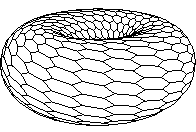
\includegraphics[width=\linewidth]{figures/torus-3d-torus.pdf}
					\caption{}
					\label{fig:torus-3d-torus}
				\end{subfigure}
				
				\caption{Visualisation of a hexagonal torus topology as a torus.}
				\label{fig:torus-3d}
			\end{figure}
			
			Figure \ref{fig:hexagonalTorusTopology} illustrates a hexagonal torus
			topology where each hexagon represents a node in the torus and touching
			edges represent connections between nodes. The nodes at the periphery of
			the system connect via wrap-around links (not shown) to nodes on opposing
			sides. To illustrate how the topology gets its name, imagine rolling the
			network into a tube such that edges $a$ and $a'$ connect. Next, bend this
			tube around forming a torus (doughnut shape), connecting $b$ to $b'$ and
			$c$ to $c'$. Note that in this paper we draw nodes as pointy-topped
			hexagons without any loss of generality: for the case where nodes are
			drawn as flat-topped hexagons, rotate the paper by 30\degree{}.
			
			Hexagonal torus topologies share many features with 2D toruses making them
			easy to reason about and describe. For example, just as in 2D toruses, the
			X- and Y- axes wrap-around single rows and columns and they form an easily
			addressed, regularly shaped system. Note that other toroidal topologies
			can be constructed with hexagonal meshes, but these are more closely
			related to twisted-torus topologies where wrapping around the X- and Y-
			axes can result in paths passing through every node in the system
			\cite{camara10}.
			
			Hexagonal topologies can be addressed by a non-orthogonal coordinate
			system through which Manhattan paths approximate Euclidean distances much
			more closely than square topologies. It is this property that gives
			hexagonal toruses their improved bisection bandwidth over 2D toruses and
			makes them popular as grids in board and computer games \cite{patel15}.
		
		\subsection{Router micro-architecture}
		\subsection{Application work-flow}
